%
% BUS 314: Resourcing New Ventures - A Course Overview
%
% Author: Jeffrey Leung
%

\documentclass[10pt, oneside, letterpaper, titlepage]{article}

\usepackage{amsmath}
\usepackage[ampersand]{easylist}
	\ListProperties(
		Progressive*=5ex,
		Space=5pt,
		Space*=5pt,
		Style1*=\textbullet\ \ ,
		Style2*=\begin{normalfont}\begin{bfseries}\textendash\end{bfseries}\end{normalfont} \ \ ,
		Style3*=\textasteriskcentered\ \ ,
		Style4*=\begin{normalfont}\begin{bfseries}\textperiodcentered\end{bfseries}\end{normalfont}\ \ ,
		Style5*=\textbullet\ \ ,
		Style6*=\begin{normalfont}\begin{bfseries}\textendash\end{bfseries}\end{normalfont}\ \ ,
		Style7*=\textasteriskcentered\ \ ,
		Style8*=\begin{normalfont}\begin{bfseries}\textperiodcentered\end{bfseries}\end{normalfont}\ \ ,
		Hide1=1,
		Hide2=2,
		Hide3=3,
		Hide4=4,
		Hide5=5,
		Hide6=6,
		Hide7=7,
		Hide8=8 )
\usepackage{geometry}
	\geometry{margin=1.2in}
\usepackage{graphicx}
	\graphicspath{ {img/} }
\usepackage[colorlinks=true, linkcolor=blue]{hyperref}
\usepackage{lmodern} % Allows the use of symbols in font size 10; http://ctan.org/pkg/lm
\usepackage{textcomp} % Allows the use of \textbullet with the font
\usepackage{verbatim}

\renewcommand{\arraystretch}{1.2}
\renewcommand{\familydefault}{\sfdefault}

\title{BUS 314: Resourcing New Ventures \\\medskip \Large A Course Overview}
\author{Jeffrey Leung \\ Simon Fraser University}
\date{Spring 2020}

\begin{document}

	\maketitle
	\tableofcontents
	\clearpage

	%
% CMPT 213: Object Oriented Design in Java - A Course Overview
% Section: Introduction
%
% Author: Jeffrey Leung
%

\section{Introduction}
	\label{sec:introduction}
\begin{easylist}

& Standards:
	&& Make fields private when possible

& Commenting:
	&& Comment purpose of a class
	&& Name fields/methods/parameters so comments are unnecessary

& When possible, convert strings to non-string types internally for consistency

& \textbf{Clean code:} Code which is correct, easy to read/maintain, and conforms to a standard

& Software design:
	&& 4 steps:
		&&& Requirements
		&&& Design and implementation
		&&& Verification
		&&& Evolution
	&& Designing involves identifying classes, responsibilities, and relationships to create a diagram
	&& Implementation process options:
		&&& \textbf{Skeleton code:} Beginning minimal parts/features of a system
		&&& \textbf{Component-wise:} Creating components one at a time
	&& Methods of integrating code from multiple people:
		&&& \textbf{Continual integration:} Gradual system growth by constantly integrating changes
		&&& \textbf{Big Bang integration:} Building all parts separately without integrating until the end

& \textbf{Feature envy:} Characteristic of a class which relies heavily on another class
& Warning sign: Characteristic of a method which operates more strongly on another object than its own
& \textbf{Deprecation:} State where a public interface is no longer supported or recommended, and is slated to be removed in the future


& \textbf{try-catch:} Structure which watches for an exception and handles it
	&& Only one exception can be live at a given time
	&& \textbf{finally clause:} Optional clause after catch clauses which is executed regardless of the result
		&&& If exception is thrown, the finally clause is executed immediately afterwards
	&& \textbf{try-with-resources:} Block which cleans up a resource when a try block exits

& Exception: Issue which may be fixable and is not out of the software's control
	&& \textbf{Checked exception:} Exception which must be caught or listed in a throws clause
	&& \textbf{Unchecked exception:} Exception which will automatically propagate and does not require catching
		&&& E.g. RuntimeException
		&&& Preferred as it does not require modification of methods between try/catch, which decouples code

\end{easylist}
\clearpage

	%
% BUS 314: Resourcing New Ventures - A Course Overview
% Section: Pitch Frameworks
%
% Author: Jeffrey Leung
%

\section{Pitch Frameworks}
	\label{sec:pitch-frameworks}
\begin{easylist}

& Positioning statement:
	&& For (target customers)
	&& Who (have a certain problem)
	&& Our product is a (description)
	&& That provides (unique breakthrough capability)
	&& Unlike (competition)
	&& Our product/solution (has a competitive differentiation)

& Components of a pitch:
	&& Market story: Description of the problem and job in the context of the market
		&&& Define the market
		&&& Examine trends
		&&& Address problems
		&&& Understand alternatives
		&&& Define an ideal solution to discuss inevitability
	&& Company story: Description of solution and competition, and the relative positioning
		&&& \textbf{Four Question Framework (4QF):} What problem is being solved, for whom, why better than the alternative, and why now?
		&&& What you belive in the company
		&&& How the company helps users
		&&& Trigger phrases: Phrases which imply underlying beliefs and thoughts
	&& Economic story: Description of the business model and return on investment
		&&& Business model
		&&& Financials/unit economics
		&&& Cpitalization structure/plans

& \textbf{Situation Complication Resolution:} Framework
	&& Situation (what): Current situation accepted as fact
	&& Complication (so what): Reason why there is a problem which needs action
	&& Resolution (now what): Action(s) required to solve the problem

& \textbf{\href{https://www.sequoiacap.com/article/writing-a-business-plan/}{Sequoia pitch}:} Pitch framework by Sequoia Venture Capital
	&& \textbf{Company purpose:} Define company in a single sentence
		&&& Communicate mission
		&&& Don't list features
	&& \textbf{Problem:} Customer pains and current methods of addressing, and shortcomings
	&& \textbf{Solution:} Unique and compelling value proposition, eventual goal
	 	&&& Discuss relevant trends
	&& \textbf{Why now:} Statement of why it is the right time for the product to enter the market
	&& \textbf{Market potential:} Identify customer and market
	&& \textbf{Competition/alternatives:} Direct and indirect competitors, and differentiation
	&& \textbf{Business model:} Discussion of the company will survive and thrive financially
	&& \textbf{Team:} Discussion of the founders and key team members
	&& \textbf{Vision:} What is the goal in several years

\end{easylist}
\clearpage

	%
% BUS 314: Resourcing New Ventures - A Course Overview
% Section: Financials
%
% Author: Jeffrey Leung
%

\section{Financials}
	\label{sec:financials}
\subsection{Basics}
	\label{subsec:financials:basics}
\begin{easylist}

& Measures:
	&& \textbf{Stock measure:} Current value held at a given time
	&& \textbf{Flow measure:} Change in a value over time

& \textbf{Liability:} Obligation to a creditor
& \textbf{Asset:} Tangible resource held
& \textbf{Equity:} Assets which may have liabilities attached
	&& Equation: Value of equity = assets - liabilities

& \textbf{Revenue/income:} Money generated
	&& \textbf{Sales/operating revenue:} Money generated from operations
	&& \textbf{Non-operating revenue:} Money generated which is not from an operation (e.g. investment interest)

& \textbf{Expense:} Money spent
	&& \textbf{Cost of Goods Sold (COGS):} Direct cost of production (e.g. materials, labor)
	&& \textbf{Non-manufacturing/Operating expense:} Expense not directly associated with productions (e.g. employee benefits)

& \textbf{Profit:} Difference between total revenue and total expenses

& \textbf{(Financial) capital:} Funds available to be used for production
	&& \textbf{Working capital:} Assets available to pay off liabilities (difference between total liabilities and total assets)

& \textbf{Accounts Receivable:} Revenues which are agreed but have not yet been received
	&& Are assets

\end{easylist}
\subsection{Balance and Income Sheet}
	\label{subsec:financials:balance-and-income-sheet}
\begin{easylist}

& \textbf{Balance sheet:} Stock measure which contains information about assets, liabilities, equity
	&& Represents the value of all assets and their method of financing (debt/equity) at a point in time
	&& Used to:
		&&& Examine liquidity
		&&& Determine financial flexibility
	&& Basis for return on equity/assets, DSO, inventory turnover, etc.
		&&& \textbf{Days Sales Outstanding (DSO):} Average number of days to collect payment after sale
			&&&& Ideal when low
	&& Total assets is equal to total liabilities plus stockholders' equity
	&& Example: See figure~\ref{img:balance-sheet-example}

\end{easylist}
\begin{figure}[!htb]
	\centering
	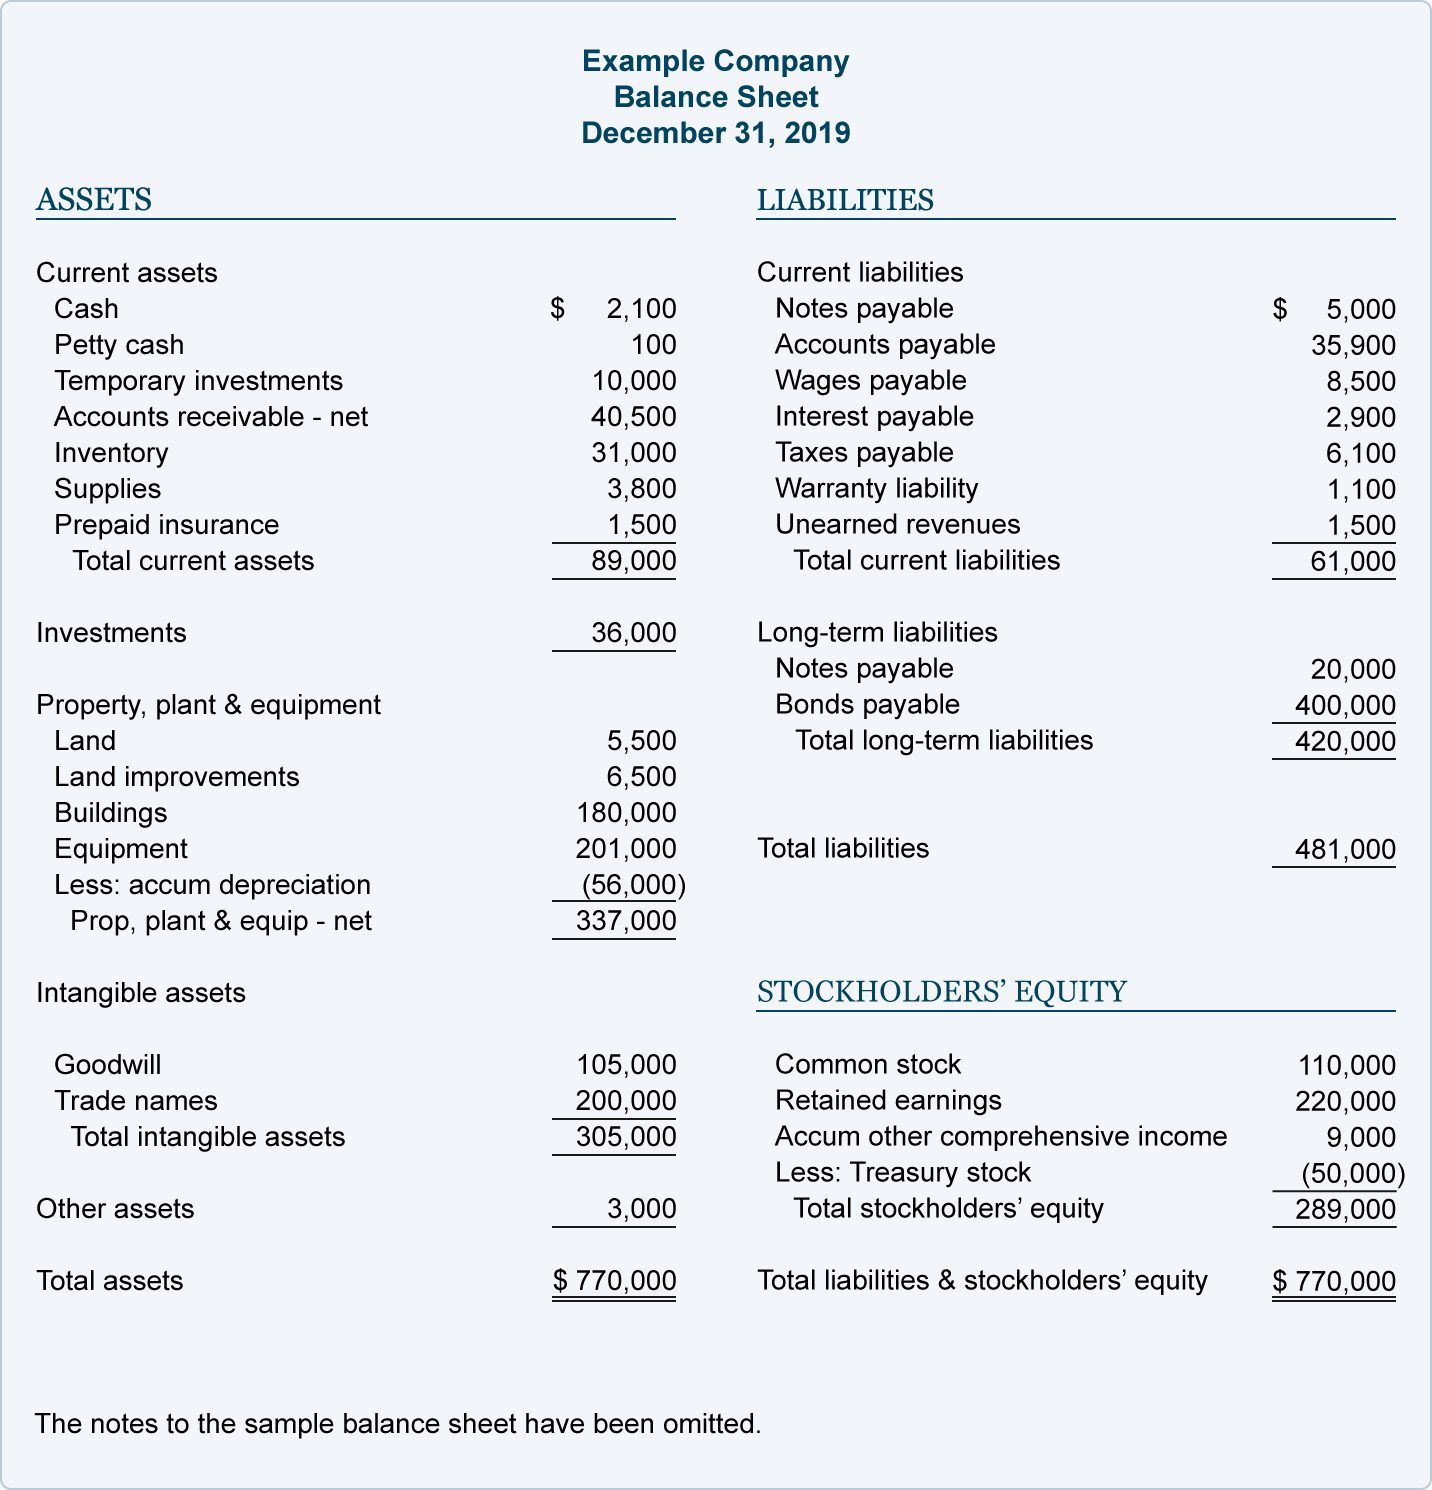
\includegraphics[width=.8\linewidth]{balance-sheet}
	\caption{Example of a Balance Sheet}
	\label{img:balance-sheet-example}
\end{figure}
\begin{easylist}

& \textbf{Income statement:} Flow measure which contains revenues, expenses, profit/income
	&& Represents the change in financial impact of operations over time
	&& Used to:
		&&& Evaluate past financial performance
		&&& Predict future cash flows
	&& Does not analyze:
		&&& Cash flow
		&&& Currently available funds
	&& Basis for gross/operating/net margin
	&& Example: See figure~\ref{img:income-statement-example}

\end{easylist}
\begin{figure}[!htb]
	\centering
	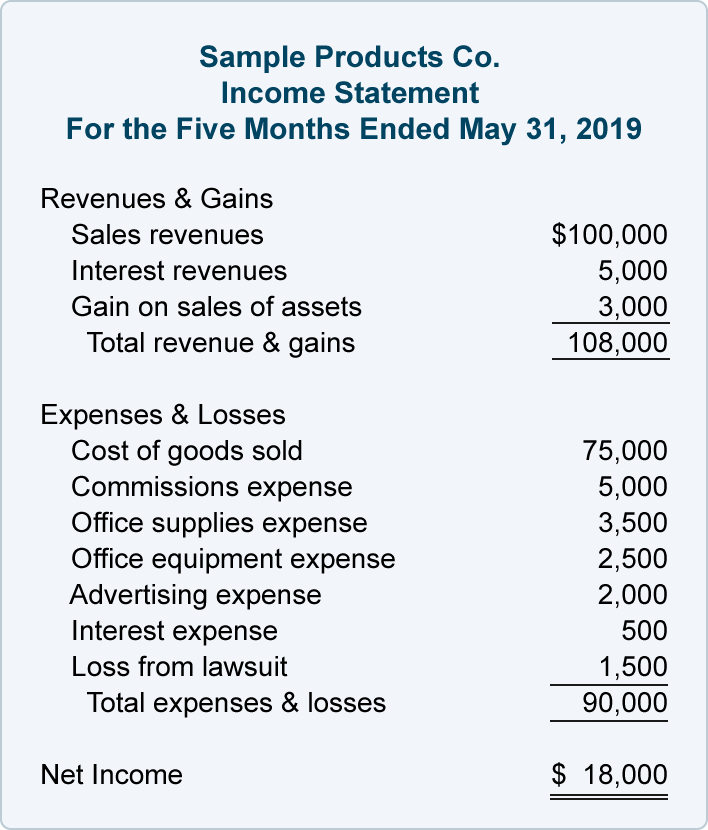
\includegraphics[width=.6\linewidth]{income-statement}
	\caption{Example of an Income Statement}
	\label{img:income-statement-example}
\end{figure}

\subsection{Financial Ratios}
	\label{subsec:financials:financial-ratios}
\begin{easylist}

& Categories of ratios:
	&& \textbf{Profitability ratio:} Proportional difference between profits over time or against other entities (e.g. gross vs. net margin)
	&& \textbf{Activity ratio:} Measure of efficiency of use of assets (e.g. DSO)
	&& \textbf{Liquidity ratio:} Measure of the ability to pay its liabilities when due (e.g. current ratio)
	&& \textbf{Coverage ratio:} Measure of the ability to meet financial obligations (e.g. months of cash burn in bank)

& Ratios:
	&& The greater, the better

	&& \textbf{Gross (profit) margin:} Difference measure which is the sales revenue minus cost of goods sold
		&&& Represents how efficiently a company creates its product

	&& \textbf{Operating margin:} Ratio measure which is (sales revenue minus operating costs) divided by sales revenue
		&&& Less than the gross margin
		&&& Represents how efficiently a company absorbs operating costs

	&& \textbf{Net (profit) margin:} Ratio measure which is net income divided by sales revenue
		&&& Less than the operating margin
		&&& Represents baseline of how much revenue per dollar is translated into profit

	&& \textbf{Return on assets:} Profitability measure which is (asset turnover times profit per asset)

\end{easylist}
\subsection{Cash Flow}
	\label{subsec:financials:cash-flow}
\begin{easylist}

& Consume cash when you:
	&& Increase assets (e.g. buying equipment)
	&& Decrease liabilities (e.g. paying back a loan, paying a supplier faster)
& Generate cash when you:
	&& Decrease assets (e.g. reducing inventory/accounts receivable)
	&& Increase liabilities (e.g. getting a loan)
	&& Issue equity (e.g. sell shares)
& No effect on cash when you:
	&& Change depreciation estimates

& \textbf{Cash flow statement:} Flow measure which contains operating, investing, and financing cash flow and the business activity which generated it
	&& For each line item, information contains: Source, amount, difference
	&& Example: See figure~\ref{img:cash-flow-statement-example}

\end{easylist}
\begin{figure}[!htb]
	\centering
	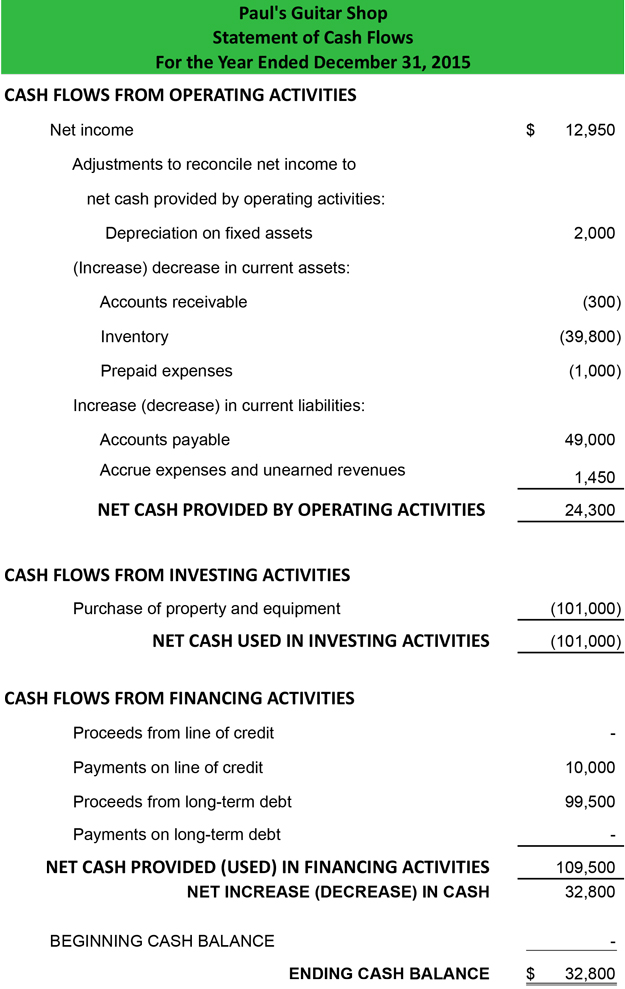
\includegraphics[width=.6\linewidth]{cash-flow-statement}
	\caption{Example of a Cash Flow Statement}
	\label{img:cash-flow-statement-example}
\end{figure}

\subsection{Balanced Scorecards}
	\label{subsec:financials:balanced-scorecards}
\begin{easylist}

& \textbf{Scorecard:} Perspective to view the health of an entity which has both a goal and an entity
	&& \textbf{Measure:} Method of quantifying a value
	&& \textbf{Goal:} Qualitative objective

& 4 scorecards:
	&& \textbf{Financial perspective:} Financial health
	&& \textbf{Customer perspective:} Customer interest and retention in the product
	&& \textbf{Internal business perspective:} Ability to efficiently and effectively deliver product
	&& \textbf{Learning/growth perspective:} Ability to innovate and continually create value

\end{easylist}
\subsection{Miscellaneous Concepts}
	\label{subsec:financials:miscellaneous-concepts}
\begin{easylist}

& Operating expenses do not include cost of goods sold

& \textbf{Insolvency/bankruptcy:} State where the value of the assets are less than the value of the liabilities

& Goodwill: Additional money paid in a purchase above valuation

& Profit can be manipulated by changing estimates/assumptions such as:
	&& Amortization of assets over longer/shorter periods of time
	&& Cpitalizing R\&D so it does not appear on the income statement

& \textbf{Unit economics:} Revenue or profit from one unit of a product/service
	&& Example of application: Number of units which must be sold to cover fixed costs
	&& Examples of metrics: Monthly active users (MAU), active revenue per user (ARPU)

& \textbf{Triple Buttom Line (3BL/TBL):} Measurement system across social, environmental, and financial aspects

\end{easylist}
\subsection{Equity}
	\label{subsec:financials:equity}
\begin{easylist}

& Multiple rounds of share distribution

& \textbf{Intellectual property:} Concept, knowledge, and technology which is the property of an entity (person, company, etc.)




\end{easylist}
\clearpage

	%
% BUS 314: Resourcing New Ventures - A Course Overview
% Section: Teams and Human Resources
%
% Author: Jeffrey Leung
%

\section{Teams and Human Resources}
	\label{sec:teams-and-human-resources}
\begin{easylist}

& \textbf{Intellectual property:} Idea, concept, or creation owned by an individual or entity
	&& Employees list prior inventions on a contract

& \textbf{Non-soliciation clause:} Legally binding clause which states an employee cannot leave a company and actively recruit their previous employees

& \textbf{Non-disclosure agreement (NDA):} Legally binding clause which states an employee cannot publish confidential information revealed to them by an entity

& \textbf{Non-compete clause (NCC):} Legally binding clause which states an employee cannot work in competition against an entity for a given amount of time

\end{easylist}
\clearpage

	%
% BUS 314: Resourcing New Ventures - A Course Overview
% Section: Capitalization Structure
%
% Author: Jeffrey Leung
%

\section{Capitalization Structure}
	\label{sec:capitalization-structure}
\subsection{Introduction}
	\label{subsec:capitalization-structure:introduction}
\begin{easylist}

& \textbf{Capitalization structure:} Distribution of debt and equity in a company

& \textbf{Venture capital:} Private equity funding provided to startups at early funding rounds

& \textbf{Stock/share:} Equity in an entity

& \textbf{Vesting:} Gradual transfer of legal ownership of equity
	&& \textbf{Cliff:} Period of time until which no shares vest
	&& \textbf{Accelerated vesting:} Ability to increase the speed at which shares vest

& \textbf{Security:} Order of reimbursement of assets during liquidation
	&& In order of most security to least security:
		&&& Debtors
		&&& Preferred shareholders
			&&&& Series B shareholders
			&&&& Series A shareholders
		&&& Common shareholders

& \textbf{Pre-money valuation:} Valuation of a company before funding

& \textbf{Post-money valuation:} Valuation of a company after funding
	&& Equation: Pre-money valuation + value of funding

& \textbf{Valuation:} Perceived balance of risk and reward

& \textbf{Pro-rata ownership:} Ability to maintain a certain percentage of ownership of the company by being given the option to purchase more shares upon any dilution

& \textbf{Term sheet:} Formal document between an investor and investing company containing terms on which investment occurs
	&& May have legally binding provisions (e.g. confidentiality)
	&& Not legally binding; does not imply a closed deal

& \textbf{Key control terms:} Contract terms to manage risk
	&& E.g. Protective provisions, anti-dilution provisions
	&& \textbf{Drag-along rights:} Contract term where a majority of voters can override the minority
	&& Control provisions exist for voting, which can be majority or super majority

& \textbf{Investment memo:} Confidential internal documentation about a decision on a potential investment

\end{easylist}
\subsection{Common Stock}
	\label{subsec:capitalization-structure:common-stock}
\begin{easylist}

& \textbf{Common stock:} Stock which has claim to assets/dividends, and gives voting rights

& Does not have a participation cap

& Calculation of common stock liquidation:
\end{easylist}
\begin{align*}
	\textrm{Common stock liquidation }
	& = \textrm{ Percent of ownership } \times \\
	& ( \textrm{Total liquidated } - \textrm{ Preferred stock liquidation} )
\end{align*}
\begin{easylist}

\end{easylist}
\subsection{Preferred Stock}
	\label{subsec:capitalization-structure:types-of-preferred-stock}
\begin{easylist}

& \textbf{Preferred stock:} Stock which has higher claim to assets/dividends than common stock, but has no voting rights
	&& Convertible to common stock at a 1-to-1 ratio

& \textbf{Series A round:} First significant round of venture capital financing
	&& \textbf{Series A stock:} Preferred stock generated during the Series A round

& \textbf{Series B round:} Second significant round of venture capital financing
	&& \textbf{Series B stock:} Preferred stock generated during the Series A round

& Investors can follow the rules for preferred stock, or convert it to common stock which removes the rules

& \textbf{Liquidation preference:} Term on preferred stock which provides guaranteed investor protection by returning liquidated proceeds first if a venture fails
	&& Calculated as a multiple of the investment
	&& Above 1x is unreasonable
	&& E.g. Given an investment of \$1M, a liqudation preference of 2x, and a liquidation of \$5M (at least greater than \$2M), the investor is guaranteed a return of \$2M

& \textbf{Participation cap:} Maximum amount of liquidated proceeds received from preferred stock, relative to the investment
	&& E.g. Given an investment of \$1M and a participation cap of 3x, the maximum amount received upon liquidating the preferred stock and participating is \$3M

& \textbf{Participating (preferred) stock:} Preferred stock which receives liquidated proceeds (investment times liquidation preference) first, then continues to receive a percentage of common stock

	&& Calculation of participating preferred stock liquidation:
\end{easylist}
\begin{align*}
	\textrm{Participating preferred liquidation } =
	& \textrm{ } MAX( \\
	& \qquad MIN( \\
	& \qquad \qquad \textrm{Investment } \times \textrm{ LiquidPref } + \\
	& \qquad \qquad \textrm{ParticipatingPrefStockPercent } \times \textrm{ TotalLiquidated}, \\
	& \qquad \qquad \textrm{Investment } \times \textrm{PartCap} \\
	& \qquad ), \\
	& \qquad toCommon(\textrm{PrefStock}) \\
	& )
\end{align*}
\begin{easylist}

& \textbf{Non-participating (preferred) stock:} Preferred stock which receives liquidated proceeds (investment times liquidation preference) but does not receive a percentage of common stock

	&& Calculation of non-participating preferred stock liquidation:
\end{easylist}
\begin{align*}
	\textrm{Non-participating preferred liquidation } =
	& \textrm{ } MAX( \\
	& \qquad MIN( \\
	& \qquad \qquad \textrm{Investment } \times \textrm{ LiquidPref }, \\
	& \qquad \qquad \textrm{Investment } \times \textrm{PartCap} \\
	& \qquad ), \\
	& \qquad toCommon(\textrm{PrefStock}) \\
	& )
\end{align*}
\begin{easylist}

& Steps to calculate exit value for a given investor with preferred shares:
	&& Calculate the value of liquidating common shares:
		&&& Change the class of shares from preferred to common, keeping the percentage the same
		&&& Multiply the percentage of common share by the liquidation amount
	&& Calculate the value of liquidating preferred shares:
		&&& Take the original investment
		&&& Multiply it by the liquidation preference
		&&& Cap it by the liquidation amount
		&&& If participating, add the participating value:
			&&&& Take the liquidation amount
			&&&& Remove the preferred share liquidation
			&&&& Multiply it by the percentage of preferred shares
			&&&& Add this to the preferred share liquidation amount calculated above
		&&& Apply the participation cap:
			&&&& Multiply the original investment by the participation cap
			&&&& Cap the liquidation amount above by this amount
		&&& Take the larger value of this vs. the value of liquidating common shares

& \textbf{Participation right:} Term where investors receive additional returns according to cap table percentage upon liquidation

& Avoid:
	&& \textbf{Redemption right:} Term which provides investors with the ability to withdraw the investment
	&& Milestone/tranching-based financing: Ability to hold back investments until a certain date or milestone
	&& Reciprocal contract

\end{easylist}
\subsection{Stock Options}
	\label{subsec:capitalization-structure:stock-options}
\begin{easylist}

& \textbf{Stock option:} Right to buy common stock (at a discounted rate)
	&& Rate to purchase is set when first issued
	&& Not stock/shares, so they cannot vote
	&& Can be converted to common shares
	&& Will vest over time

& Stages in the capitalization table:
	&& Reserved
	&& Allocated
	&& Vested
	&& Exercised

& \textbf{Exercise/strike price:} Discounted price at which a share can be bought using a stock option

\end{easylist}
\subsection{Stages}
	\label{subsec:capitalization-structure:stages}
\begin{easylist}

& \textbf{Startup:} Venture which has not yet received Series B funding
	&& Financing from equity (initial investors), customers, employees (who will work for equity and lower salary)

& \textbf{Scaling:} Venture which has received Series B funding but is not yet public or having private equity
	&& Financing from equity, debt, and customers

& \textbf{Mature:} Venture which is stable, being public or having private equity
	&& Financing from equity, debt, and customers

\end{easylist}
\clearpage


\end{document}
